\title{Supplementary Material for the HMRS manuscript}
\begin{document}
\maketitle


\noindent\textbf{Reading the supplementary material.} The material is
grouped by evidence type, and each result retains the corpus and unit
reported in the main text. Figure~S1 shows the service boundaries and
shared state. Figures~S2--S3 report answer-marker and out-of-corpus probe
observations; Figures~S4--S5 replay verifier roles and illustrate one
logged query. Table~S9 indexes the management checks, Table~S10 summarises
the retrieval and answer designs, and Table~S11 positions representative
research strands. Tables~S12--S13 give arm counts and paired contrasts for
E5. The reruns reuse the same in-domain questions on later corpus states.
Tables~S14--S16 retain the
question-level answer proxies, aggregate answer and runtime observations,
and the DeepSeek-R1 answer-case comparison. For the 72 in-domain questions,
a post-hoc check lowercased each question and its nonempty annotated target,
then tested exact substring containment without other normalization. The
29 overlapping questions had frozen containment of 16/29 for A0 and 21/29
for A0h; the other 43 had 21/43 and 31/43, respectively. These non-random
subsets are descriptive, not a causal test, and other lexical cues may remain
in the non-overlap group. Table~S17 records the design
and provenance of every campaign named in the main text. Tables S1--S8 of
the companion inventory document (shipped alongside this supplement)
complete the campaign-level evidence index. Each trace CSV
packages 76 question IDs per complete arm. The in-domain analyses exclude the
four out-of-domain probes R1--R4.

\begin{figure}
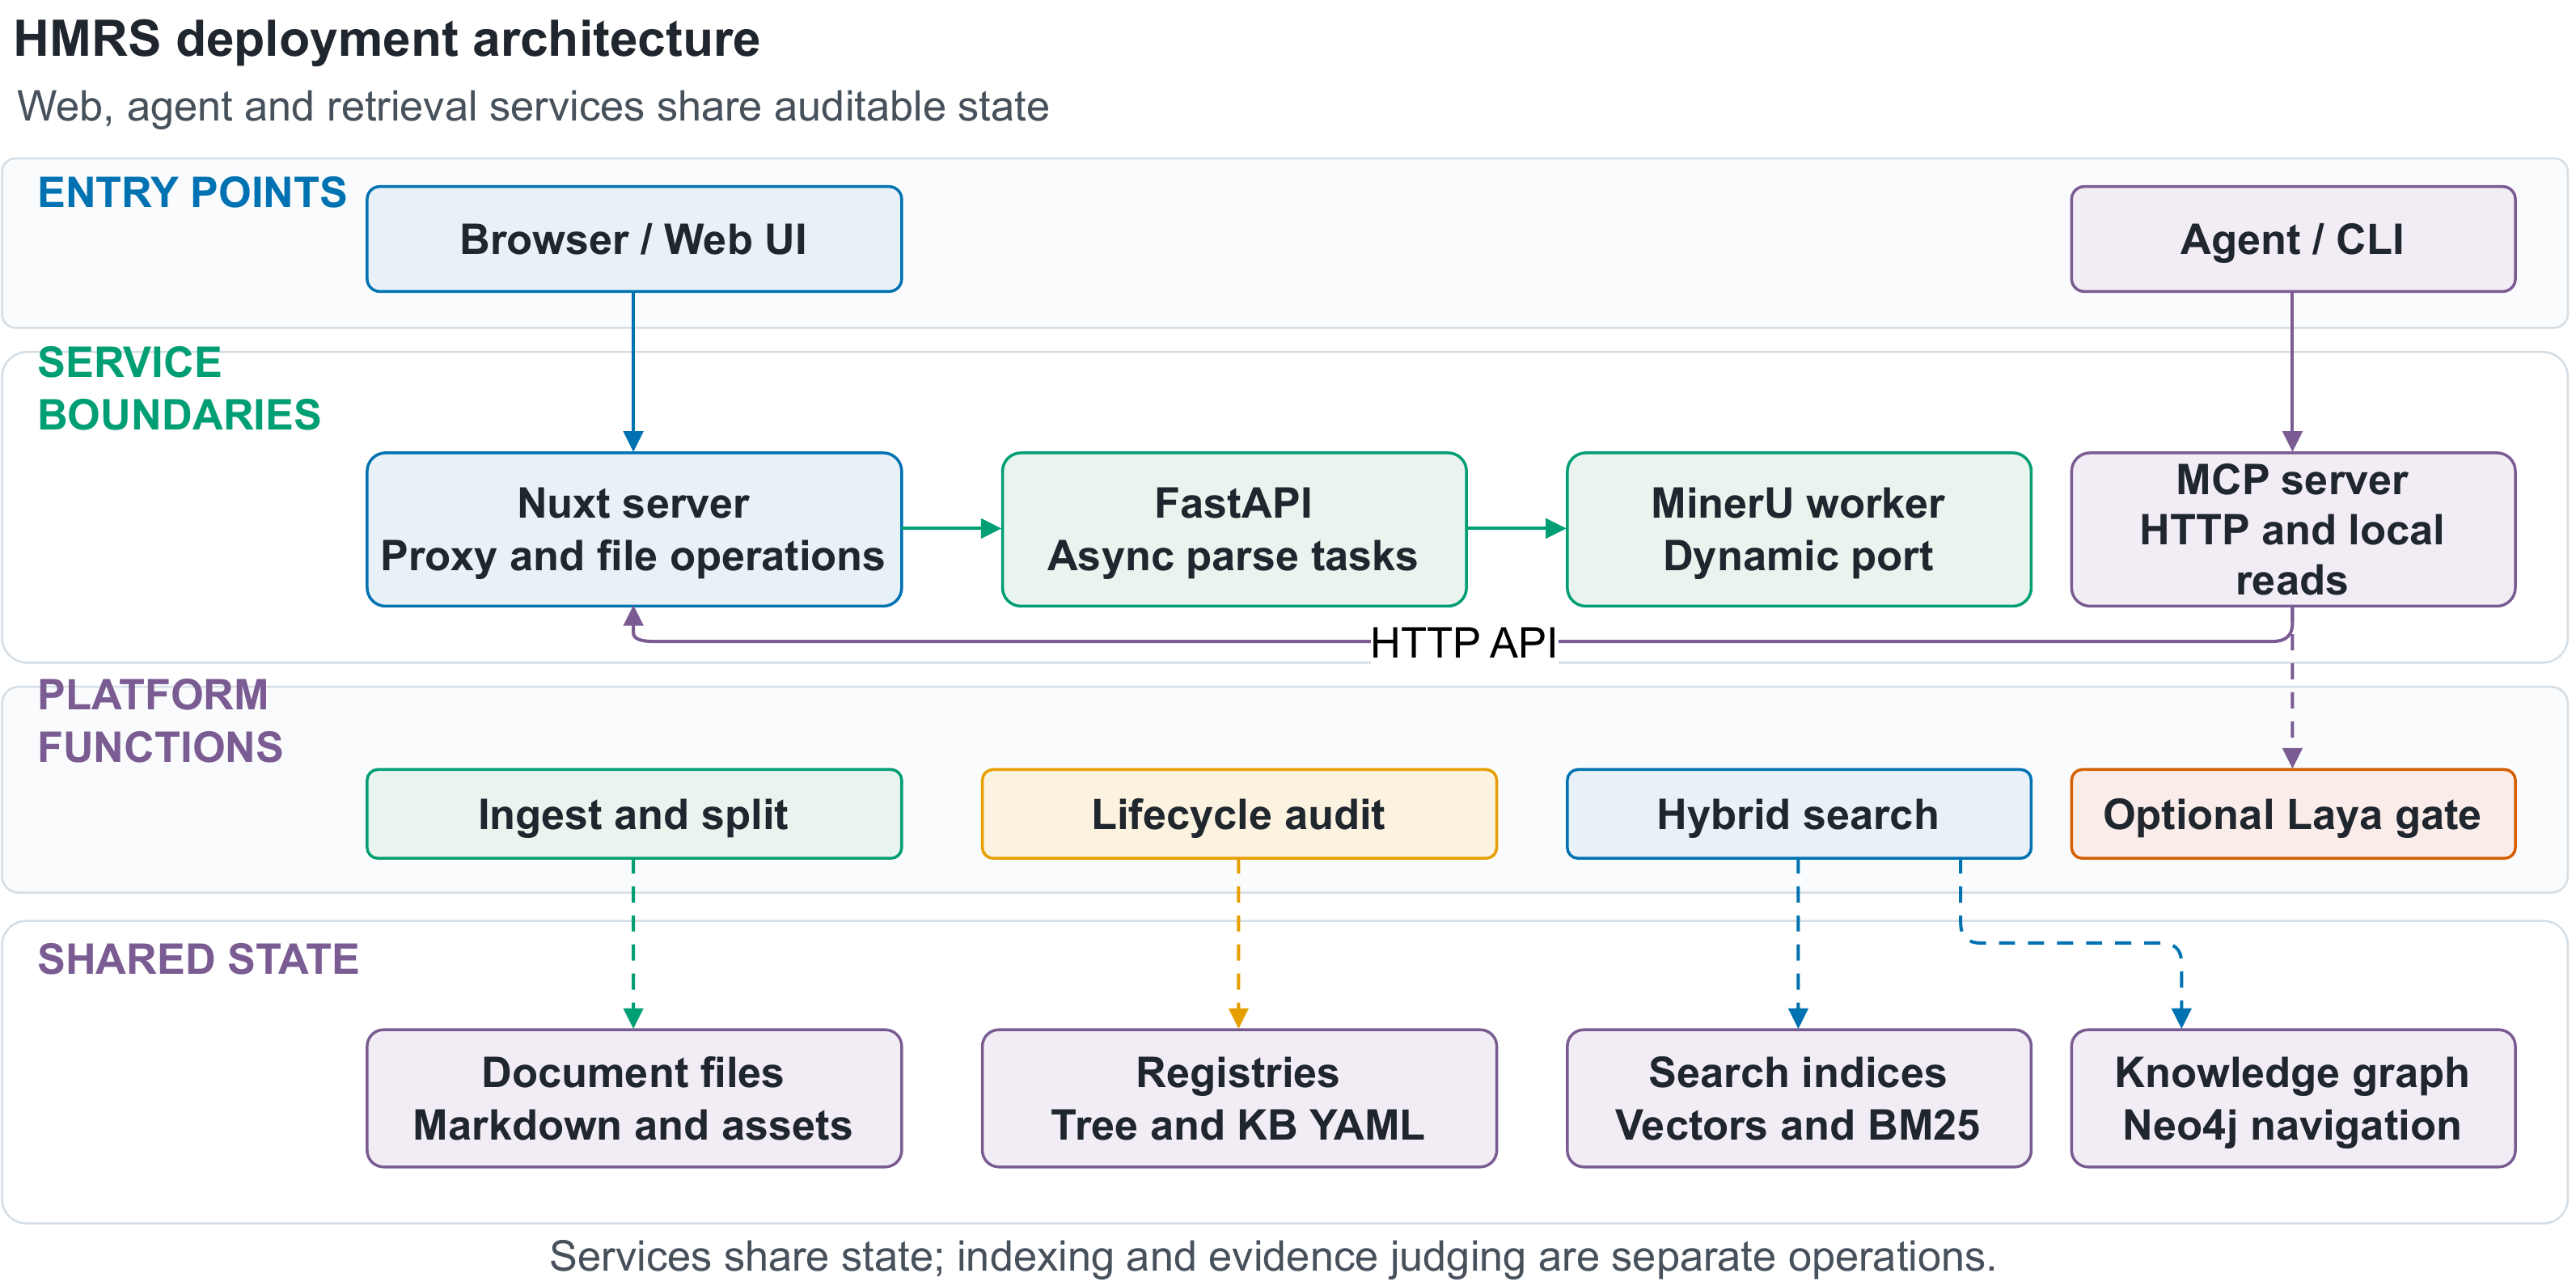
\includegraphics[width=6.45in]{figs/fig1_architecture_native.png}
\caption{\textbf{Figure S1.} HMRS service boundaries and shared state. The browser
reaches the Nuxt server, and agent tools use the MCP server. The evidence
gate is an optional call.}

\end{figure}
\begin{figure}
\centering
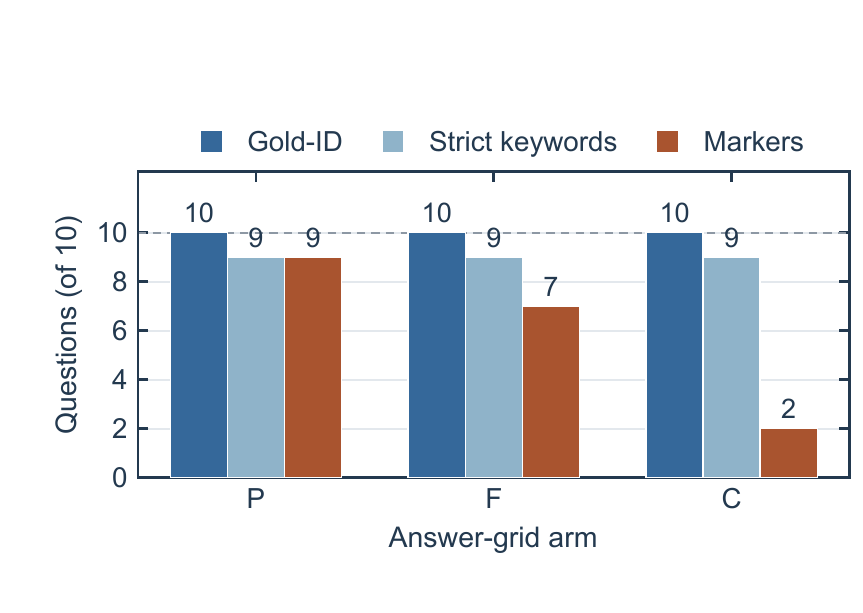
\includegraphics[width=4.1in]{figs/fig_opt_s_answer.png}
\caption{\textbf{Figure S2.} Answer checks for the original grid (30 cells,
\texttt{run-20261013T094350Z-5f9faac}). P = platform agent, F = file
tools, C = 800-character chunk replica. Gold-identifier coverage is at
ceiling in all three arms; strict keyword coverage shows three misses, and
recognised citation markers fall from nine to seven to two answers. A later
grid on selected libraries gives nine marker-bearing answers in every arm;
its C arm used the same five libraries and a different substrate. The
marker pattern counts document-style syntax; it does not verify citation
resolution or claim support. Wall-clock and cost figures for these cells
are reported in Table~S15. The common-substrate rerun changed BQ06's
question, so it is not a fully matched question set.}

\end{figure}
\begin{figure}
\centering
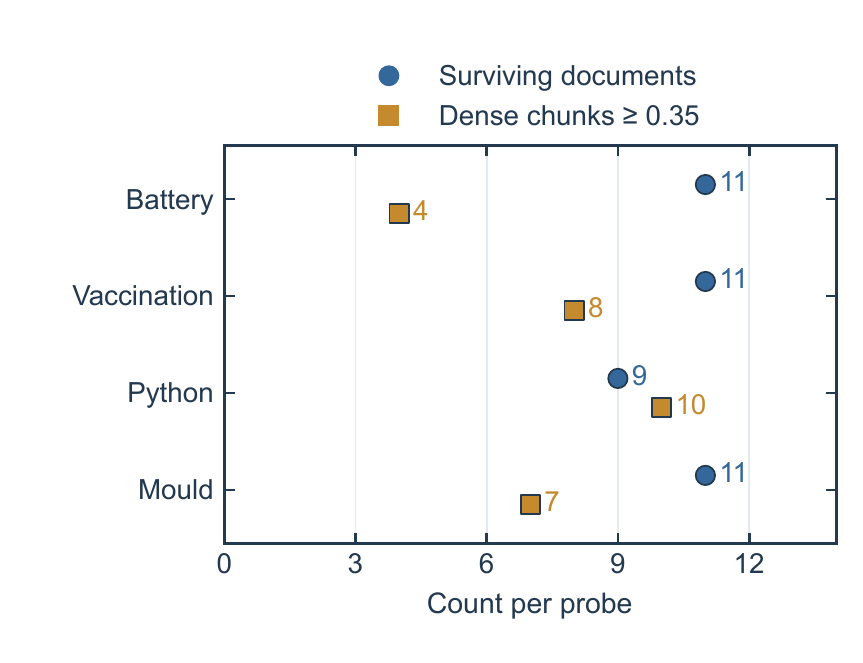
\includegraphics[width=4.1in]{figs/fig_exp_s3.png}
\caption{\textbf{Figure S3.} Tool-layer out-of-corpus probes
(\texttt{paper-kbs/experiments/results/exp3\_abstention.json}) retained
9--11 documents after the 12-candidate cap; the merged pool had 42--43
candidates. Separately, dense-search chunks had scores above the 0.35
threshold. The two counts use different units (documents versus chunks).
Thus the retrieval threshold did not identify semantic absence in these
probes. In a separate answer-workflow probe family
(\texttt{paper-kbs/experiments/results/exp8b\_absent\_agent.json}),
three completed absent queries returned natural-language not-found reports
and no fabricated citation was observed. The latter is an observation of
instructed agent behaviour, not a server-side guarantee.}

\end{figure}
\begin{figure}
\centering
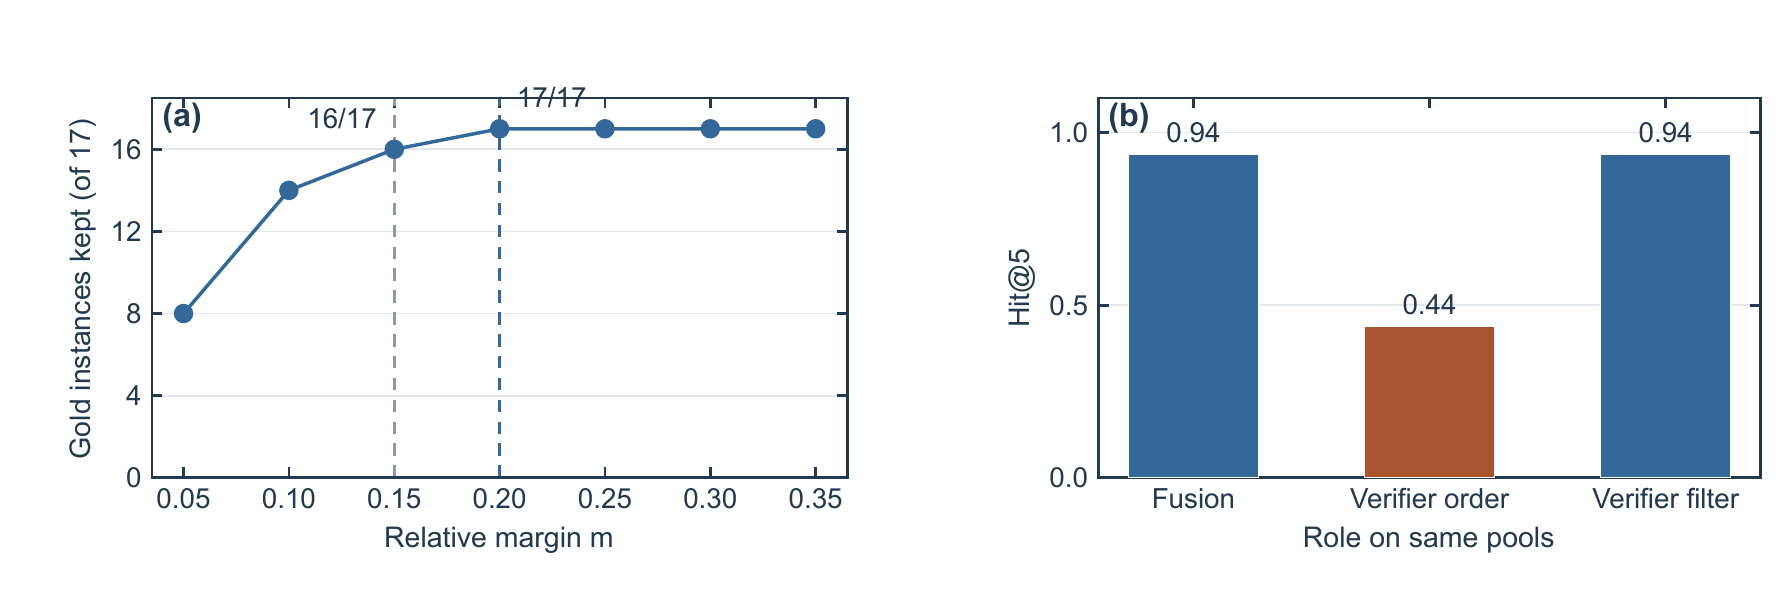
\includegraphics[width=6.45in]{figs/fig_opt_s_margin.png}
\caption{\textbf{Figure S4.} Two replays over the logged hybrid pools analysed in the main
paper's verifier section; both reuse recorded candidate pools and verdict
scores rather than retrieving again. (a)~A relative-margin replay: keep the
top five plus every candidate within $m$ of the pool's best score, $m$
swept 0.05--0.35; the curve counts gold instances kept of the 17 that
entered a pool; dashed rules mark $m=0.15$ (16 of 17) and $m=0.20$ (all
17); the mean candidate count rises from 6.4 to 11.9 of the twelve
submitted. (b)~Verdict roles on identical candidates and identical scores:
fusion order, verdict order and verdict filter; only the role differs, which
makes the panel an attribution rather than a benchmark; the verdict-order
role loses the gold, while the filter role leaves the fusion order intact.
Hit@5 is 0.94, 0.44 and 0.94.}

\end{figure}
\begin{figure}
\centering
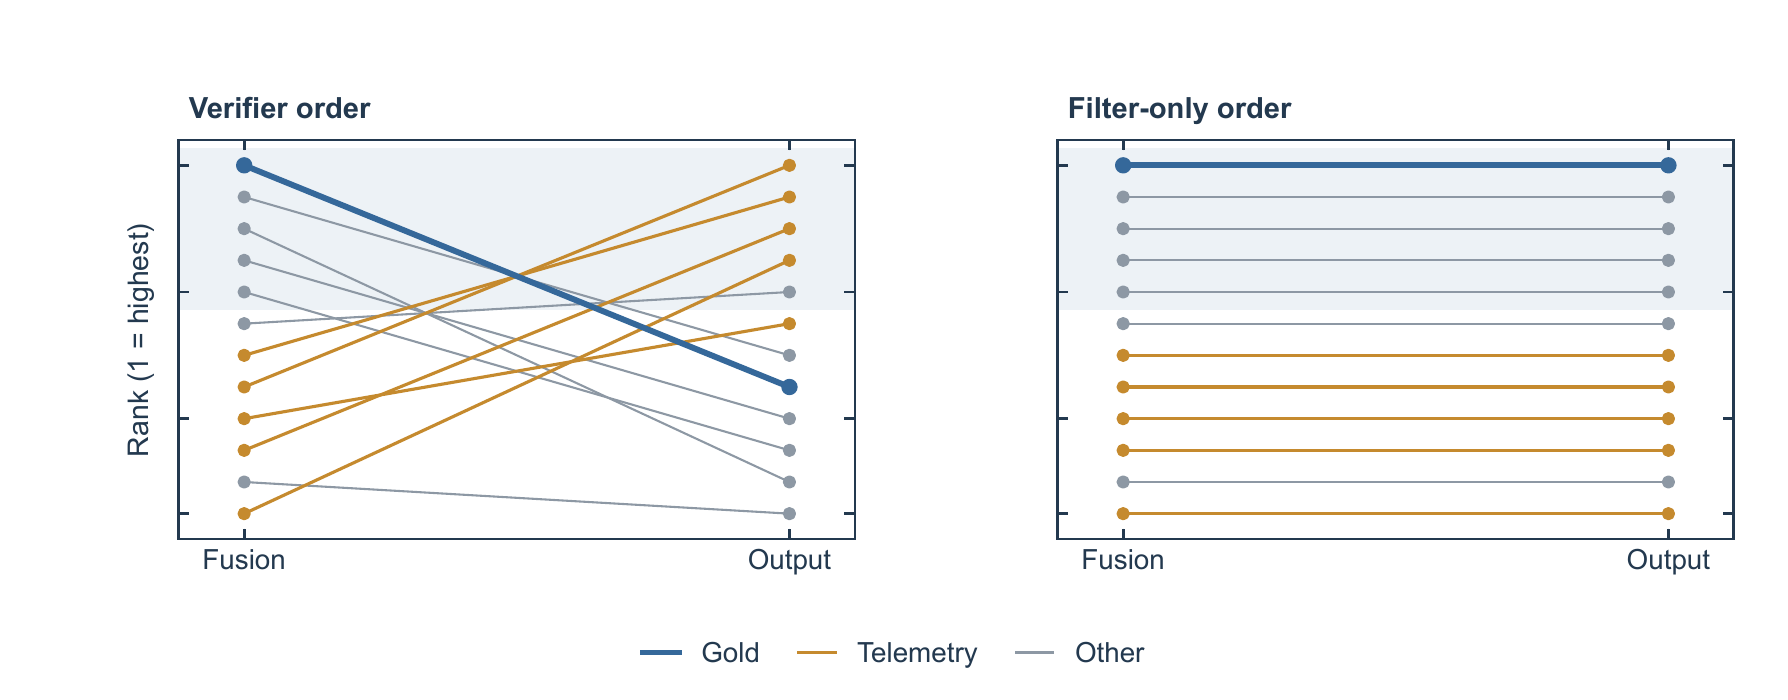
\includegraphics[width=6.45in]{figs/fig_exp_s5.png}
\caption{\textbf{Figure S5.} Anatomy of one real query (Q2; single logged HMRS-Hybrid call).
Each line is one of the 12 fused candidates; the shaded band is the top-5
window selected for source reading in the recorded run. (a)~In the logged
re-ranking, the
judge scores five extruder-PLC telemetry reports $0.887$--$0.926$ and the
gold root-cause report $0.846$, demoting it from fusion rank~1 to
rank~8 --- outside the read window. (b)~The same call with the verdicts
used only as a filter: all 12 pass, the fusion order stands, and the gold
is the first document read. Same pool, same scores, same verdicts; only
the role of the induced ordering differs.}

\end{figure}
\begin{table}
\centering
\footnotesize
\setlength{\tabcolsep}{4pt}
\caption{\textbf{Table S9.} Functional checks on the management layer. Each row names the
function, the test and its scale, the observed outcome, and the subsection
that reports it. The numbers are those of the cited campaigns; none is
re-estimated. A passing check means the stated property was observed on the
stated scale, not that the function is exhaustively verified.}

\begin{tabular}{@{}p{1.898cm}p{4.373cm}p{6.435cm}p{1.650cm}@{}}
\toprule
Function & Test and scale & Observed outcome & Where\\
\midrule
Parse and ingest & 100-paper target; November disk inventory & Each target had at least one stored part. Earlier records contain 91 state-list names and 79 documents enumerated and read in a derived library; these are not a matched funnel and have no reliable shared audit date & E1\\
Description audit & November re-check across five libraries & 328/328 parts had descriptions of at least 60 characters without the recorded placeholder pattern; six parts were non-target. The 100-ID short-query probe is diagnostic: 72 searches were unscoped and 45 returned a chunk-copy name first & E1\\
Parse quality & 50-paper, 26-domain campaign & 50/50 parsed and verified, all probes ok; 202 tags; 41 tag flags negative without blocking ingestion & E1\\
Structural split & 50 papers at the 30{,}000-character tier & 165 stored parts (9 whole papers, 156 split parts) in 2{,}672\,s; storage 50/50; descriptions and tags 165/165 & E1\\
Near-duplicate review & 322-part corpus, 0.90 threshold & 35 candidate groups (0.90--0.975), zero true duplicates, nothing deleted & E2\\
Campaign inventories & Separate five-library inventory and 400 Wikipedia pages per language & 322 parts in the five-library inventory, not a count of the target papers. Expected titles in preassigned libraries: 350/400 (en), 400/400 (zh, ja) & E1--E2\\
Content audit and three-source consistency & 322-part inventory; 33-part storage sample & 322/322 archived content snippets nonempty, each at most 1,000 characters; 33/33 sampled storage checks across files, tree and metadata; separate rename defect fixed by re-index & E2\\
Lifecycle operations & 16 scenarios on two disposable libraries & create, move, delete and forced re-index pass; two failures (task status, update check) & E2\\
Sub-library hierarchy & Three-level disposable fixture & create, parent-to-child move, listing, reading and judging all pass & E2\\
Tags and graph & 316-tag registry; 658-node graph & 165 stored parts pass the tag check in 47.6\,s; four tag edges on one document move 4{,}675 to 4{,}679 & E2\\
Experience store & One heuristic smoke run; one separate case report & 13 draft creations reported; a later top-ranked retrieval is report-level only, with its successful raw response unavailable; the empty-pool approval check did not exercise approval & E4\\
\bottomrule
\end{tabular}
\end{table}
\begin{table}
\centering
\footnotesize
\setlength{\tabcolsep}{4pt}
\caption{\textbf{Table S10.} Design and headline results of the retrieval and answer experiments.
Each row names the corpus and scale, the metric and the comparison it is read
against, the headline outcome, and the claim that outcome supports together
with its limit. Tables~S12--S13 give the campaign-level E5 counts and paired
contrasts.}

\begin{tabular}{@{}p{1.650cm}p{3.300cm}p{3.960cm}p{3.960cm}p{2.145cm}@{}}
\toprule
Exp & Corpus and scale & Metric and comparison & Headline result & Supports / limit\\
\midrule
E3 (RQ2) & Ten-domain 72 q; route cards with and without descriptions & Scripted gold-domain choice & A0 72/72 vs nominally name-only A3 37/72; McNemar $p=5.82\times10^{-11}$ & Scripted probe, unlogged fallback; configuration contrast, not a causal description effect\\
E5 (RQ3) & 72 questions in ten domains across three campaigns & Target-string containment, text volume and paired exact McNemar tests & A0h vs A0: 52/72 vs 37/72 frozen, 51/72 vs 39/72 in the first follow-up, 48/72 vs 36/72 on November 17 & Configuration contrasts on the same set. A0h--PD remains unresolved in the frozen and first follow-up records.\\
E6 (RQ5) & Two 30-cell grids, three interfaces; later 10-question run & Gold-ID in answer or trace, lexical coverage, citation markers & Gold-ID 60/60 at ceiling; markers 9/7/2 (original), 9/9/9 (common substrate); separate post-repair tiered run 10/10 under a broader marker rule & Grid questions lack gold IDs; BQ06 changed in the common grid; marker rules differ for the later run. ID and markers do not establish source support; one run per arm\\
E7 (RQ5) & Three arms $\times$ three questions, public API & Cost, refusal behaviour, transport & Question Q2 false refusal on a 131-doc catalogue (74.9\,KB over tool budget); repaired by pagination & Transport and cost boundary; one campaign plus replication\\
E8 (RQ4) & 191 logged scores and a separate ordering archive & Gold vs non-gold scores and same-pool Hit@5 & Median scores 0.88 vs 0.86 ($p=0.26$). Hit@5 was 7/16 in verifier order and 15/16 in fusion order. & Historical wrapper and one corpus.\\
E9 & 27-cell stability; 90/180/270-request read sweep; separate vector-only trial; gate on/off $n=10$; pinned vs unscoped scope & Wall clock and completion within observation window; answer grades; Hit@5 under each scope & Read sweep recorded no errors; in the separate vector trial 111/270 were unfinished at 30 seconds; no measured gate benefit here; gold-pinned Hit@5 1.0 (non-gold 0.0) & Single-instance envelope; unfinished requests are not established timeouts; scope not isolated, filename confound\\
\bottomrule
\end{tabular}
\end{table}
\begin{table}
\centering
\small
\setlength{\tabcolsep}{4pt}
\renewcommand{\arraystretch}{1.18}
\caption{\textbf{Table S11.} Positioning. Each strand addresses part of the path from stored
document to answer. HMRS studies a knowledge document management workflow
combining automatic collection assignment, content-informed acquisition,
server-side checks when invoked, and answer-layer reporting; the evaluation
measures selected components and boundaries in the main paper. References for
the representative strands are provided in the main paper's related-work section.}

\begin{tabular}{@{}p{2.392cm}p{4.702cm}p{3.960cm}p{3.960cm}@{}}
\toprule
Strand & Representative work & What it optimises & What it leaves to the deployment\\
\midrule
Knowledge management & Public knowledge bases; enterprise content management & An explicit ontology, or governance over a curated collection & Whether an answer drawn from that collection is supported by the text it cites\\
Document AI & Layout-aware extraction; MinerU & Recovery of text, tables and formulas from difficult layouts & Whether what was recovered is complete enough to index, and where it is then stored\\
Retrieval & Dense, lexical and hybrid ranking & Rank quality over a corpus that is assumed indexed & Whether a top-ranked candidate contains evidence for the claim it is used to support\\
Graph-structured organisation & GraphRAG, LightRAG, RAPTOR & Multi-hop and hierarchical relationships between documents & Evidentiary status: a graph edge is a navigation fact, not evidence\\
Self-reflective generation & Self-RAG, CRAG, FLARE; judge-based verification & Evidence assessment or retrieval correction in generation workflows & How verification and abstention interact with knowledge-base acquisition and organisation in a knowledge-base workflow\\
Agentic tool use & ReAct, MCP & Access to retrieval tools behind a stable interface & Whether configured retrieval budgets and failure states are exposed and checked in a particular deployment\\
Structure-aware navigation & DeepRead  & In-document section coordinates for locate-then-read agentic search & Cross-collection lifecycle governance and selected reconciliation audits\\
Collection selection & CORI, ReDDE & Ranking collections by estimated relevance before within-collection search & Lifecycle governance and three-source reconciliation of the selected collections\\
\midrule
HMRS (this work) & Main paper, Sections 3--7 & A management-level model: automatic collection assignment, three-source state checks, a tiered access path, an invoked server-side evidence gate and agent answer reporting & Claims beyond the measured corpora and configurations, bounded in the main paper limitations\\
\bottomrule
\end{tabular}
\end{table}
\begin{table}
\centering\small
\caption{\textbf{Table S12.} Annotated target-string containment in returned evidence packs on 72
in-domain questions across three recorded campaigns. A target
occurrence in a sibling document may count, so this is a lexical proxy rather
than gold-document retrieval or answer correctness. Wilson intervals describe
the frozen counts. Agreement compares the first follow-up with the frozen
run. The November 17 run used the live corpus after a service restart and
reused the existing route-card libraries for A3. Mechanical read-all was
incomplete in the first follow-up and omitted on November 17. Arms
differ in more than one component and some reference lookups may use the gold
domain.}

\begin{tabular}{lrrrrrr}
\toprule
Configuration & Frozen & Frozen rate & Wilson 95\% CI & Follow-up & Agreement & Nov.\ 17 \\
\midrule
A0 & 37/72 & 51.4\% & [40.1, 62.6]\% & 39/72 & 68/72 & 36/72 \\
A0f & 45/72 & 62.5\% & [51.0, 72.8]\% & 44/72 & 71/72 & 41/72 \\
A0h & 52/72 & 72.2\% & [61.0, 81.2]\% & 51/72 & 71/72 & 48/72 \\
PD & 46/72 & 63.9\% & [52.4, 74.0]\% & 45/72 & 71/72 & 42/72 \\
A1b & 39/72 & 54.2\% & [42.7, 65.2]\% & 39/72 & 72/72 & 36/72 \\
A2 & 25/72 & 34.7\% & [24.8, 46.2]\% & 25/72 & 72/72 & 23/72 \\
A3 & 33/72 & 45.8\% & [34.8, 57.3]\% & 25/72 & 54/72 & 26/72 \\
Read-all & 72/72 & 100.0\% & [94.9, 100.0]\% & -- & -- & -- \\
\bottomrule
\end{tabular}
\end{table}
\begin{table}
\centering\small
\caption{\textbf{Table S13.} Exploratory paired annotated target-string containment contrasts in
returned evidence packs on the 72 in-domain questions (two-sided exact
McNemar tests, unadjusted; no familywise inference). The follow-up repeats the
same questions and is not an independent sample; an archived same-corpus
reproduction of the frozen content arms agreed with the frozen records on
71/72 questions for A0f, A0h and PD and on 68/72 for A0. A target occurrence
may be in a sibling document; arms differ in multiple components and some
lookups may use the gold domain.}

\begin{tabular}{llrrr}
\toprule
Run & Contrast & First only & Second only & $p$ \\
\midrule
Frozen & A0h vs. A0 & 15 & 0 & 0.000061 \\
Frozen & A0h vs. A1b & 13 & 0 & 0.00024 \\
Frozen & A0h vs. PD & 7 & 1 & 0.07031 \\
Frozen & PD vs. A1b & 7 & 0 & 0.01563 \\
Frozen & A0f vs. A0 & 8 & 0 & 0.00781 \\
Frozen & A1b vs. A0 & 4 & 2 & 0.6875 \\
Frozen & A2 vs. A0 & 6 & 18 & 0.0227 \\
Follow-up & A0h vs. A0 & 12 & 0 & 0.00049 \\
Follow-up & A0h vs. A1b & 12 & 0 & 0.00049 \\
Follow-up & A0h vs. PD & 7 & 1 & 0.07031 \\
Follow-up & PD vs. A0 & 6 & 0 & 0.03125 \\
Follow-up & A0f vs. A0 & 5 & 0 & 0.0625 \\
Follow-up & A1b vs. A0 & 1 & 1 & 1.0 \\
Follow-up & A2 vs. A0 & 5 & 19 & 0.0066 \\
Nov.\ 17 & A0h vs. A0 & 12 & 0 & 0.00049 \\
\bottomrule
\end{tabular}
\end{table}

\begin{table}
\centering
\small
\setlength{\tabcolsep}{3pt}
\caption{\textbf{Table S14.} Question-level answer proxies for the original 30-cell grid
(\texttt{run-20261013T094350Z-5f9faac}). For each arm, s is strict
keyword coverage, a is alias-aware coverage, and m is the count of
recognised citation-like markers. Original answers were rescored against the
revised BQ06 annotations; under the original annotation P's strict total is
10/10 rather than 9/10. The gold ID appeared in the answer or
trace in all cells; this check is omitted from the table. None of the saved
grid question texts contains its corresponding gold ID. The check searches
answer text and recorded tool-call inputs and agent text, and ID presence
does not establish source resolution. A marker does not
verify source resolution or entailment.}

\begin{tabular}{@{}lp{4.950cm}l*{9}{c}@{}}
\toprule
 & & & \multicolumn{3}{c}{Platform (P)} & \multicolumn{3}{c}{File (F)} & \multicolumn{3}{c}{Chunk replica (C)}\\

Q & Question (abridged) & Gold & s & a & m & s & a & m & s & a & m\\
\midrule
BQ01 & Transformer attention and recurrence & 1706.03762 & ✓ & ✓ & 6 & ✓ & ✓ & 0 & ✓ & ✓ & 5\\
BQ02 & NISQ definition and limitation & 1801.00862 & ✓ & ✓ & 4 & ✓ & ✓ & 3 & ✓ & ✓ & 0\\
BQ03 & MultiMedQA and Flan-PaLM on MedQA & 2212.13138 & ✓ & ✓ & 4 & ✓ & ✓ & 1 & ✓ & ✓ & 1\\
BQ04 & Gene Ontology subdivisions & 1602.01876 & ✓ & ✓ & 1 & ✓ & ✓ & 1 & ✓ & ✓ & 0\\
BQ05 & European growth and Unified Growth Theory & 1512.08067 & ✓ & ✓ & 0 & ✓ & ✓ & 0 & ✓ & ✓ & 0\\
BQ06 & Controls on precipitation extremes & 1503.07557 & $\times$ & ✓ & 6 & ✓ & ✓ & 4 & ✓ & ✓ & 0\\
BQ07 & MameLoshnLM and parameter scale & 2608.05850 & ✓ & ✓ & 1 & ✓ & ✓ & 2 & ✓ & ✓ & 0\\
BQ08 & Oxygen redox and cathode capacity & 2408.09942 & ✓ & ✓ & 2 & ✓ & ✓ & 0 & ✓ & ✓ & 0\\
BQ09 & Visual SLAM in dynamic scenes & 2410.10669 & ✓ & ✓ & 2 & $\times$ & ✓ & 6 & ✓ & ✓ & 0\\
BQ10 & Tumour control under immune evasion & 2604.01385 & ✓ & ✓ & 3 & ✓ & ✓ & 6 & $\times$ & ✓ & 0\\
\midrule
 & \emph{All ten questions} & & 9 & 10 & 29 & 9 & 10 & 23 & 9 & 10 & 6\\
\bottomrule
\end{tabular}
\end{table}
\begin{table}
\centering
\small
\setlength{\tabcolsep}{4pt}
\caption{\textbf{Table S15.} Aggregate answer and runtime proxies for the original and
common-substrate grids, plus a separate post-repair run. Lexical checks do
not establish semantic support; each arm is one run. The post-repair run is
a single current-state observation on a later stack and is not pooled with
the grids. BQ06 changed in the common-substrate rerun, and original-grid
keyword totals use revised BQ06 annotations rather than the original rule.
The post-repair
marker count uses a broader recognition rule than the grid counts and is not
directly comparable to them.}

\begin{tabular}{@{}p{3.960cm}*{4}{c}p{1.980cm}p{2.475cm}@{}}
\toprule
Grid and arm & Gold-ID & Strict & Alias & Markers & Mean time (s) & Cost (USD)\\
\midrule
Original, P & 10/10 & 9/10 & 10/10 & 9/10 & 52.6 & 0.711/q\\
Original, F & 10/10 & 9/10 & 10/10 & 7/10 & 22.2 & 0.487/q\\
Original, C & 10/10 & 9/10 & 10/10 & 2/10 & 24.5 & 0.527/q\\
Common, P & 10/10 & 7/10 & 9/10 & 9/10 & 37.7 & 0.672/q\\
Common, F & 10/10 & 7/10 & 9/10 & 9/10 & 15.2 & 0.377/q\\
Common, C & 10/10 & 8/10 & 10/10 & 9/10 & 19.6 & 0.524/q\\
Current, post-repair & 10/10 & 9/10 & -- & 10/10 & 131 & 3.10 total\\
\bottomrule
\end{tabular}
\end{table}
\begin{table}
\centering\small
\caption{\textbf{Table S16.} Recorded answer-case comparison on one ingested DeepSeek-R1 paper.
The cells summarise the case compendium; complete responses and source text
are retained in the associated demonstration records. The prompt identified
the library and paper and prescribed the tool steps. This non-blinded case
study is not a measurement of autonomous selection, general answer accuracy or
abstention.}

\begin{tabular}{@{}p{2.970cm}p{5.775cm}p{5.775cm}@{}}
\toprule
Question & OMP response summary & Claude response summary \\
\midrule
Benchmark scores & AIME 79.8\%, MATH-500 97.3\%; distinguished R1-Zero & Same two values; distinguished R1-Zero \\
RL and rewards & GRPO, rule-based rewards; noted reward hacking & GRPO and rule-based rewards; noted reward hacking \\
R1-Zero training & RL without SFT; poor readability and language mixing & RL without SFT; poor readability and language mixing \\
Electricity cost & No electricity amount reported; distinguished the \$294K rental-based training estimate & No electricity amount reported; distinguished the \$294K rental-based training estimate \\
\bottomrule
\end{tabular}
\end{table}
\begin{table}
\centering
\footnotesize
\setlength{\tabcolsep}{4pt}
\caption{\textbf{Table S17.} Evaluation design and provenance. Each row is a separate corpus, run
and unit; counts are not pooled into a system-level accuracy. The 72-question
follow-up reuses the frozen questions and reports 906 stored parts. The
November arXiv observation is a filename-stem short-query identifier probe,
not scoped title retrieval or a matched before--after comparison. The answer
grids use one run per arm and lexical proxies; the verifier score archive and
ordering archive are separate records.}

\begin{tabular}{@{}p{2.640cm}p{3.465cm}p{4.125cm}p{4.950cm}@{}}
\toprule
Campaign and state & Material and unit & Comparison or observation & Measure and boundary\\
\midrule
Industrial corpus, 2026-10-13 & 42 documents in five libraries; 16 questions & Hybrid candidates; verifier ordering & Document Hit@5; same-pool replay; one workstation\\
arXiv answer grid, 2026-10-13 & 100-paper target; 10 questions & Platform, file and chunk-replica answer arms & Gold-ID, strict/alias keywords, markers; one run per arm; the separate 322-part inventory is not a target-paper count\\
arXiv, 2026-11-14/15 & 100 targets; 328 five-library parts including six non-target parts; 10 questions & Filename-stem ID diagnostic and scoped ten-question vector check & At least one disk part per target; IDs found in probe result names; 72/100 probes unscoped, 45 chunk-copy-first; not a matched rerun\\
Wikipedia ingestion & 400 pages per language; 40 excerpt queries per language & Ingestion into preassigned English, Chinese and Japanese libraries & Expected-title coverage and a top-three self-retrieval check\\
Routing, frozen and follow-up & 72 in-domain questions; 138 documents; 879 parts (follow-up 906) & Description-layer and content-layer configurations & Gold-domain choice and annotated target-string containment in returned packs; multiple components; sibling matches may count; same questions, not independent\\
Answer grids & 10 questions; 30 cells per grid & Platform, file and chunk-replica arms; common substrate & Gold-ID, strict/alias keywords, markers; one run per arm; lexical proxies, not semantic support\\
Verifier archive & 191 scores from 16 hybrid runs; 17 gold and 174 non-gold & Score distribution and same-pool ordering & Medians and Hit@5; separate archives; exploratory $p$ values; filtering never activates\\
\bottomrule
\end{tabular}
\end{table}
\end{document}
